\documentclass[handout,nooutcomes]{ximera}
\usepackage{booktabs}
%% handout
%% space
%% newpage
%% numbers
%% nooutcomes

\renewcommand{\outcome}[1]{\marginpar{\null\vspace{2ex}\scriptsize\framebox{\parbox{0.75in}{\begin{raggedright}P\arabic{problem} Outcome: #1\end{raggedright}}}}}

\renewenvironment{freeResponse}{
\ifhandout\setbox0\vbox\bgroup\else
\begin{trivlist}\item[\hskip \labelsep\bfseries Solution:\hspace{2ex}]
\fi}
{\ifhandout\egroup\else
\end{trivlist}
\fi}

\newcommand{\RR}{\mathbb R}
\renewcommand{\d}{\,d}
\newcommand{\dd}[2][]{\frac{d #1}{d #2}}
\renewcommand{\l}{\ell}
\newcommand{\ddx}{\frac{d}{dx}}
\everymath{\displaystyle}
\newcommand{\dfn}{\textbf}
\newcommand{\eval}[1]{\bigg[ #1 \bigg]}


\title{Breakout Session 17: Graphing functions}

\begin{document}
\begin{abstract}
  \textbf{A look back:} In the previous (March 3, 2016) Breakout Session you practiced using the signs of the first and second derivatives to locate local extrema and determine intervals where the function is increasing, is decreasing, is concave up, or is concave down.

  \textbf{Overview:} In today's (March 10, 2016) Breakout Session you'll practice how to sketch the graph  of a function.
  
  \textbf{A look ahead:} In the next (March 22, 2016) Breakout Session you'll learn how to optimize using calculus.
\end{abstract}
\maketitle

\section{Learning Outcomes}
\label{section:learning-outcomes}
The following outcomes are \emph{not an exhaustive} list of the skills you will need to develop and integrate for demonstration on quizzes and exams.
This list is meant to be a starting point for conversation (with your Lecturer, Breakout Session Instructor, and fellow learners) for organizing your knowledge and monitoring the development of your skills.

\begin{itemize}
  \item
    Determine how the graph of a function looks without using a calculator.
  \item
    Understand what information the derivative gives concerning when a function is increasing or decreasing.
  \item
    Understand what information the second derivative gives concerning concavity of a function.
  \item
    Interpret limits as giving information about functions.
  \item
    Determine how the graph of a function looks based on an analytic description of the function.
  \item
    Find the intervals where a function is increasing or decreasing.
  \item
    Find the intervals where a function is concave up or down.
  \item
    Find any asymptotic behaviors a function may have: vertical, horizontal, or slant.
  \item
    Determine how the graph of a function looks without using a calculator.)
\end{itemize}
\newpage

\begin{problem}
  \mbox{}
  \begin{enumerate}
    \item[1.]
      You are given that $f''(x) > 0$ for all $x$.
      Which of the following must be true about $f(x)$ on the region $0 \leq x \leq 2$?
      \begin{enumerate}
        \item
          There is a critical point between $0$ and $2$.

        \item
          An absolute maximum occurs at either $x=0$ or $x=2$.

        \item
          There is a local maximum, but not enough information is given to determine where.

        \item
          $f$ need not have a local maximum.
      \end{enumerate}
      \begin{freeResponse}
        Only (b) and (d) must be true.
        The following picture provides a counterexample for both (a) and (c):
        \begin{image}
          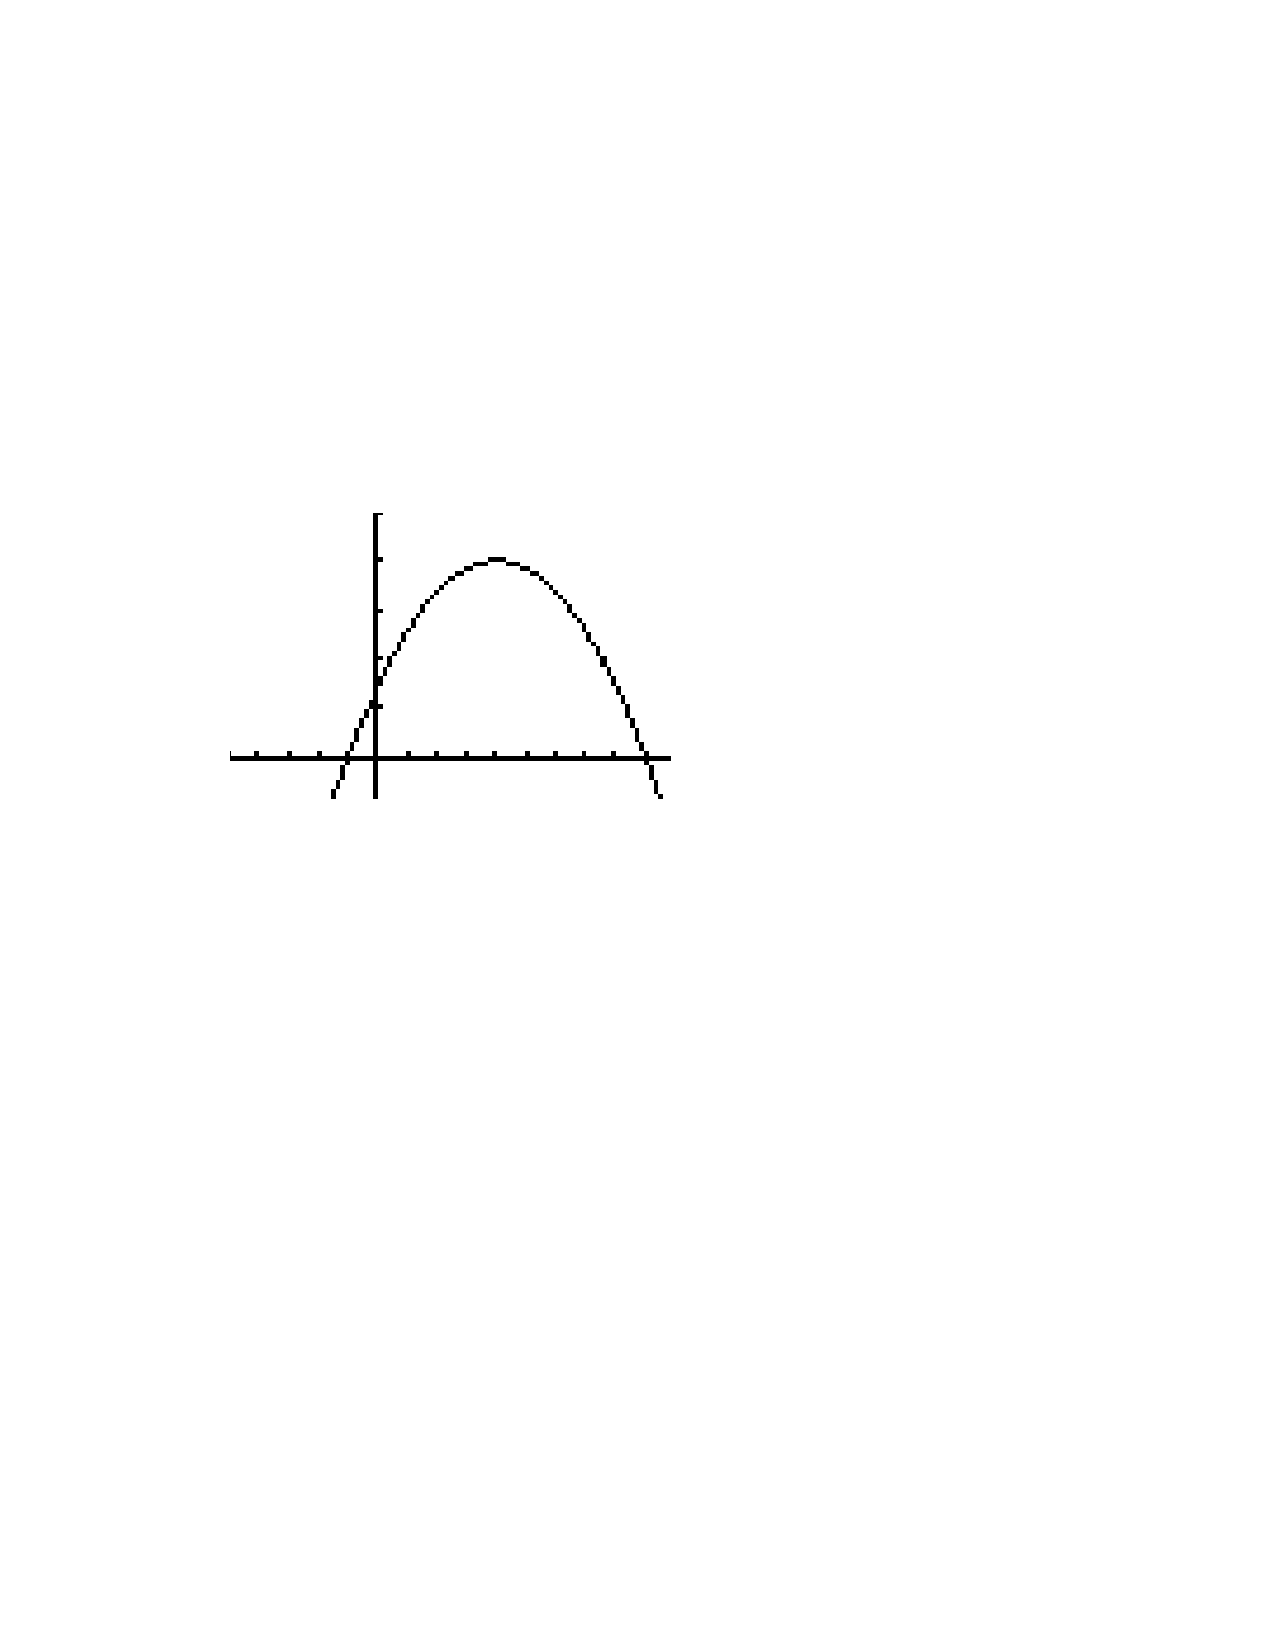
\includegraphics[trim= 70 470 250 190]{Images/Figure1.pdf}
        \end{image}
      \end{freeResponse}
		
     \item[2.]  
       You are told that $f''(x) > 0$ for all $x$.
       Which of the following must be true about the graph of $y=f(x)$?
       \begin{enumerate}
         \item
           The graph is a straight line.

         \item 
           The graph crosses the $x$-axis at most once.
         
         \item
           The graph is concave down.

         \item
           The graph crosses the $y$-axis more than once.

         \item
           The graph is concave up.
       \end{enumerate}
       \begin{freeResponse}
         Only (e) must be true.
         For (a), the function $f(x) = e^x$ provides a counterexample:
         \begin{image}
           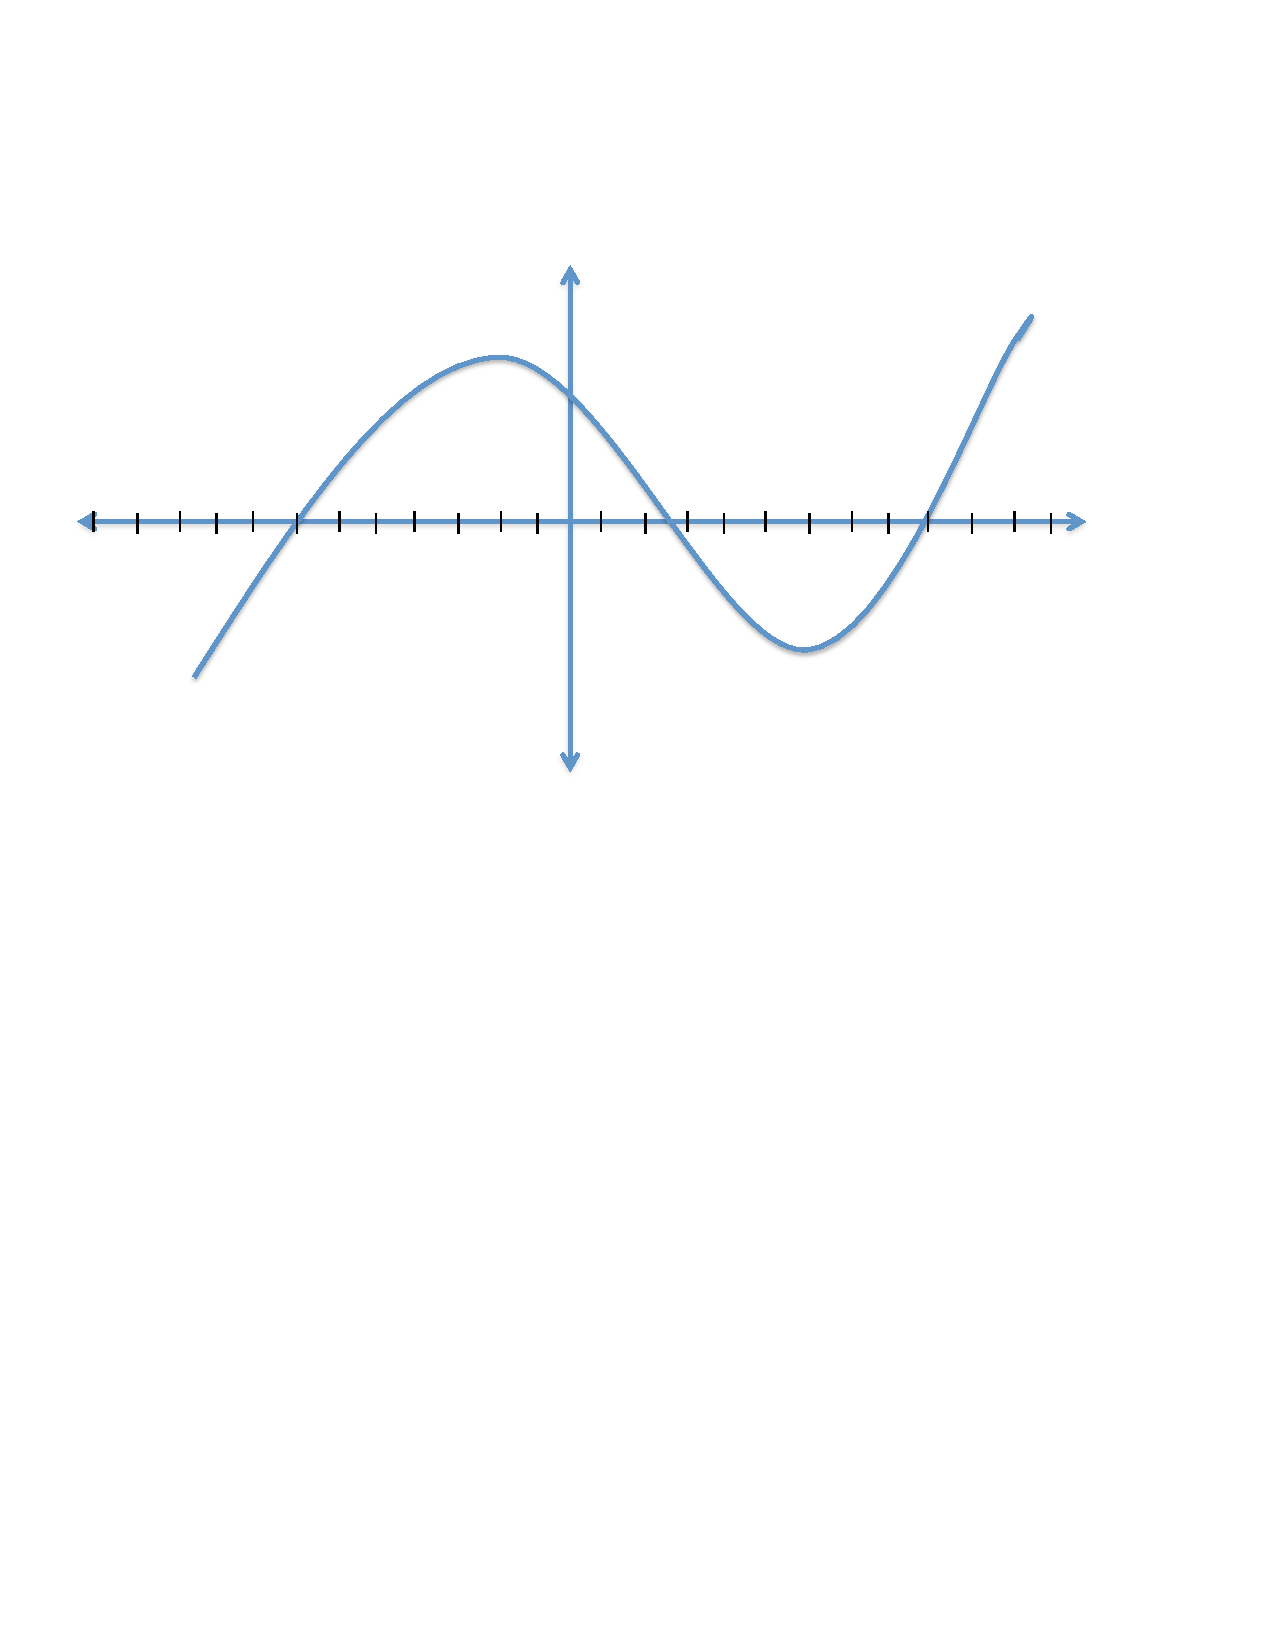
\includegraphics[trim= 70 470 250 190]{Images/Figure2.pdf}
         \end{image}
			
         For part (b), the function $f(x) = x^2 -2$ provides a counterexample:
         \begin{image}
           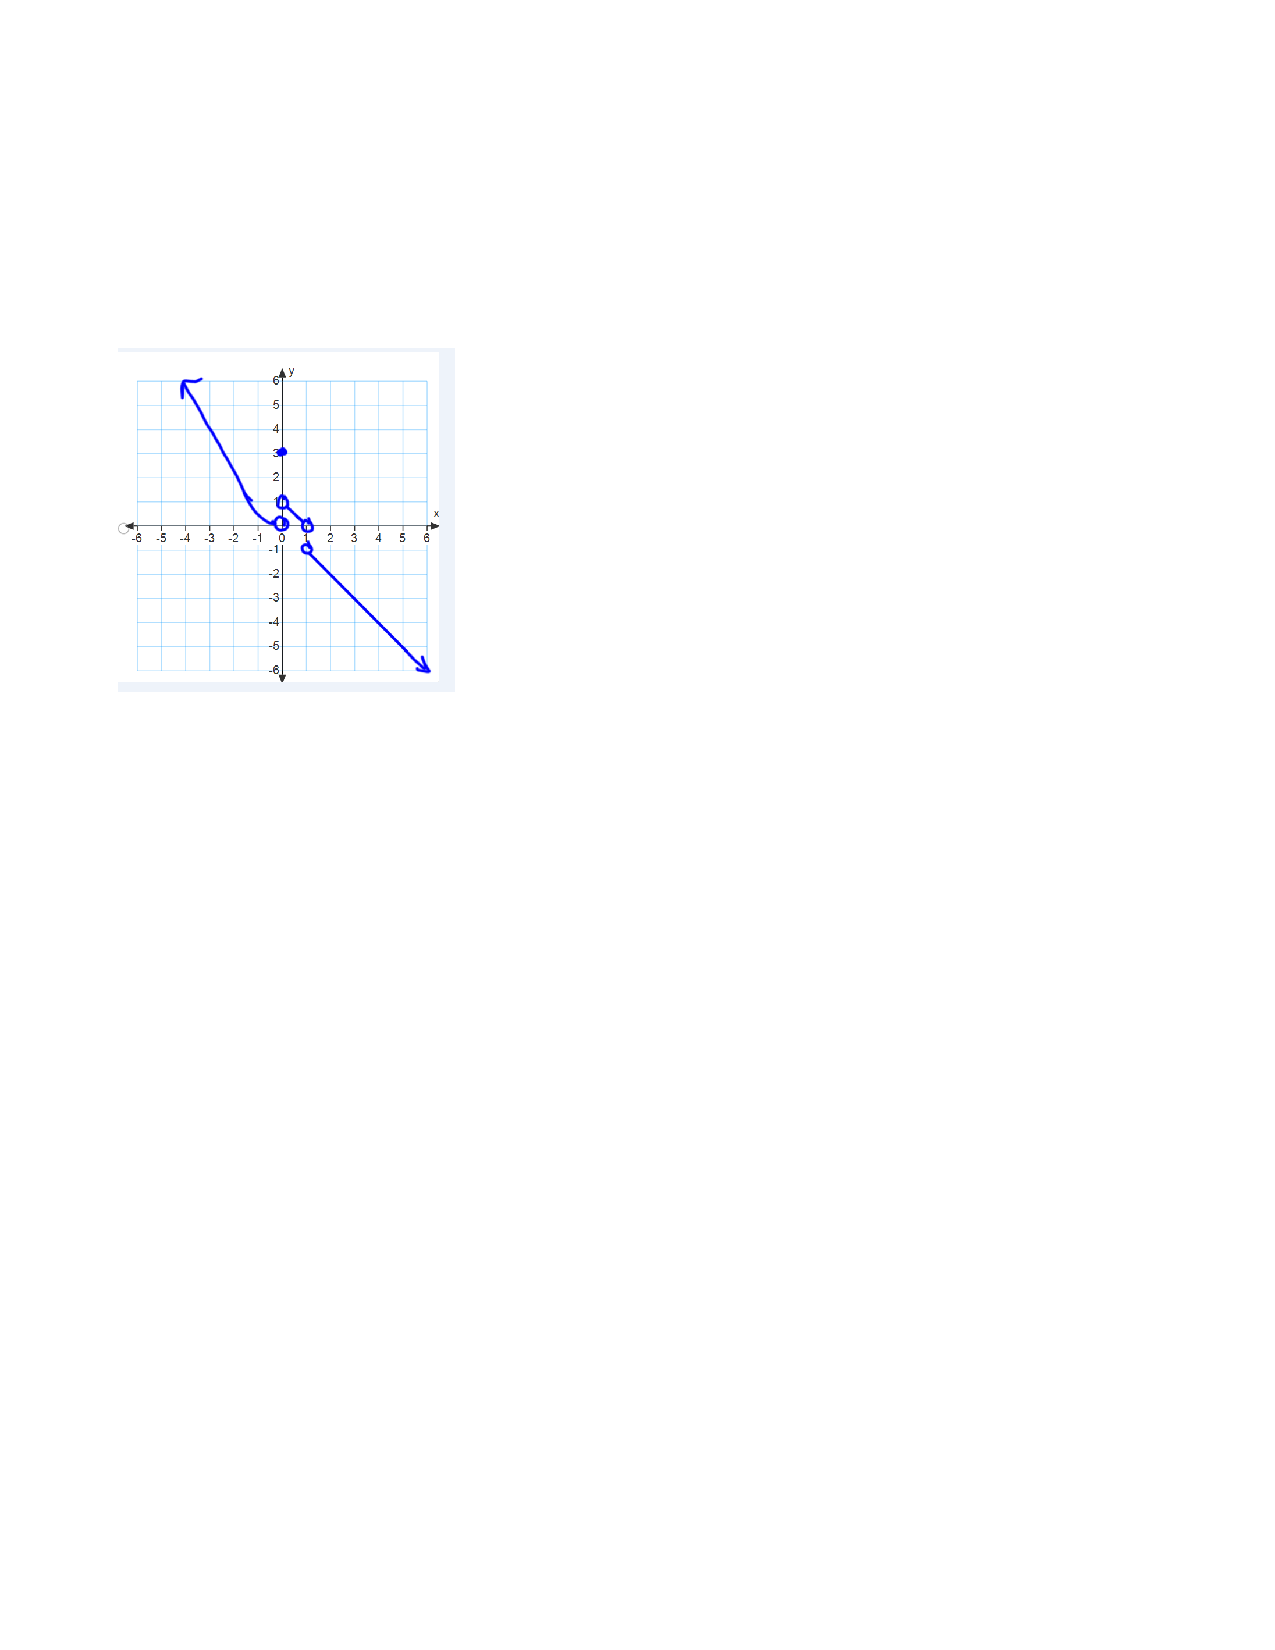
\includegraphics[trim= 70 470 250 190]{Images/Figure3.pdf}
         \end{image}
			
         Part (c) is clearly false since $f''(x) > 0$ means that $f$ is concave up.
         Part (d) is false for any function.
       \end{freeResponse}
    \end{enumerate}
\end{problem}

\begin{problem}
  Sketch (neatly!) the graph of a function $f$ satisfying all of the conditions:
  \begin{itemize}
    \item[(a)]
      $f$ is continuous and \emph{odd}, $f(0) = 0$,

    \item[(b)]
      $\displaystyle \lim_{x \to \infty} f(x) = -5$,

    \item[(c)]
      $f'(x) > 0$ on $(6, \infty)$,

    \item[(d)] 
      $f'(x) < 0$ on $(0, 6)$,

    \item[(e)]
      $f''(x) > 0$ on $(0, 12)$, and
      
    \item[(f)]
      $f''(x) < 0$ on $(12, \infty)$.
  \end{itemize}
  \begin{center}
    \begin{image}
      \includegraphics[scale = 0.07]{Images/"Blank Grid".pdf}
    \end{image}
  \end{center}
\end{problem}

\begin{problem}
  Follow all the steps on the ``Graph Sketching Summary Sheet'' and then graph the given function:
  \[ 
    f(x) = \frac{x^2 + x + 1}{x^2}
  \]
  \begin{freeResponse}
    \begin{itemize}
      \item  
        \dfn{Domain}  \\
        The function is a rational function, and so the domain of the function is all real numbers except where the denominator equals zero.
        \[
          x^2 = 0 \quad \Longrightarrow \quad x=0
        \]
	So the domain of $f$ is $(-\infty ,0)\cup (0,\infty )$.


      \item
        \dfn{$x,\, y$-intercepts}  \\
        To find any $x$-intercept(s), set $y=0$ and solve:
        \begin{align*}
          \frac{x^2 + x + 1}{x^2} = 0 &\implies x^2 + x + 1 = 0 \\
          &\implies x = \frac{-1 \pm \sqrt{1-4(1)(1)}}{2(1)}
        \end{align*}
	which has no real solutions.
        Thus, $f$ has no $x$-intercepts.
			
	Since $x=0$ is not in the domain of $f$, $f$ has no $y$-intercepts as well.
 
     \item 
       \dfn{Symmetry}  \\

       It is clear that $f$ is not periodic.
       Note that $f(1) = 3$ and $f(-1) = 1$.
       So it cannot be for all values of $x$ that either $f(-x) = f(x)$ or $f(-x) = -f(x)$.
       So $f$ is neither even nor odd, and therefore $f$ has no symmetry.
			
     \item
       \dfn{Asymptotes}  \\

       \dfn{Vertical Asymptotes:}  Our only candidate is $x=0$, and so we compute the two one-sided limits:
       \[
         \lim_{x \to 0^-} \frac{x^2+x+1}{x^2} = \infty 
       \]
       \[
         \lim_{x \to 0^+} \frac{x^2+x+1}{x^2} = \infty
       \]
       Therefore, $x=0$ is the only vertical asymptote of $f$.

       \dfn{Horizontal Asymptotes:}  We compute the following limits:
       \[
         \lim_{x \to \infty} \frac{x^2+x+1}{x^2} = 1
       \]
       \[
         \lim_{x \to -\infty} \frac{x^2+x+1}{x^2} = 1
       \]
       and so the only horizontal asymptote of $f$ is $y=1$.
			
       \dfn{Slant Asymptote:}  Since our function is rational, we need to check for slant asymptotes.
       Since the degree of the numerator is not one greater than the degree of the denominator, we do not have a slant asymptote.
			
     \item
       \dfn{Increasing/Decreasing}  \\

       \begin{align*}
         f'(x) &= \frac{x^2(2x+1) - (x^2+x+1)(2x)}{x^4} \\
               &= \frac{2x^3 + x^2 - 2x^3 - 2x^2 - 2x}{x^4} \\
               &= \frac{-x^2 - 2x}{x^4} \\
               &= \frac{-x-2}{x^3}
       \end{align*}
			
       To find where $f'$ is both positive and negative, we need to find where $f'(x) = 0$ and where $f'(x)$ does not exist.
       Clearly, $f'(x)$ does not exist when $x=0$.
       To find when $f'(x) = 0$, we solve:
       \begin{align*}
         \frac{-x-2}{x^3} = 0 &\implies -x-2 = 0 \\
         &\implies -x = 2\\
         &\implies x = -2
       \end{align*}
       Since $x=0$ is not in the domain of $f$, $x=-2$ is the only critical point of $f$.
       To see where $f$ is increasing and decreasing, consider the following sign chart for $f'$:
       \begin{center}
         \begin{image}
           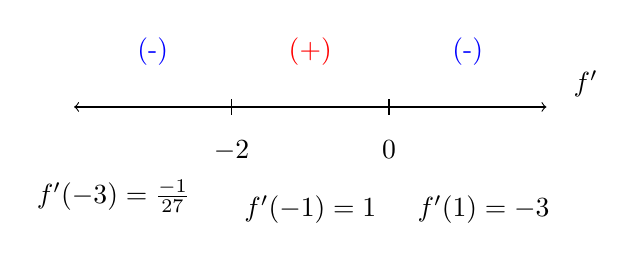
\begin{tikzpicture}
             \draw [<->] (-4,0) -- (2,0);
             \draw (0,0.1) -- (0,-0.1);
             \draw (-2,0.1) -- (-2,-0.1);
             \draw (-2,-0.3)node[below]{$-2$};
             \draw (0,-0.3)node[below]{$0$};
             \draw (-3.5,-0.8)node[below]{$f'(-3) = \frac{-1}{27}$};
             \draw (-1,-1)node[below]{$f'(-1) = 1$};
             \draw (1.2,-1)node[below]{$f'(1) = -3$};
             \draw[red] (-1,1)node[below]{(+)};
             \draw[blue] (1,1)node[below]{(-)};
             \draw[blue] (-3,1)node[below]{(-)};
             \draw (2.5,0)node[above]{$f'$};
           \end{tikzpicture}
         \end{image}
       \end{center}

       So we see that $f$ is increasing on $[-2,0)$, and $f$ is decreasing on $(-\infty, -2] \cup (0,\infty)$.
       
     \item
       \dfn{Local Extrema}  \\
       $f'$ changes from negative to positive at $x=-2$, so this is the location of a local minimum.
       $f'$ also changes from positive to negative at $x=0$, but $f$ is not defined at $x=0$ and so this is not a local extreme value.
       $f$ has a local minimum at $\left( -2,\frac{3}{4} \right)$.
			
			
			
     \item
       \dfn{Concavity}
       \begin{align*}
         f''(x) &= \frac{x^3(-1) - (-x-2)(3x^2)}{x^6} \\
                &= \frac{-x^3 + 3x^3 + 6x^2}{x^6} \\
		&= \frac{2x^3 + 6x^2}{x^6} \\
		&= \frac{2x+6}{x^4} \\
		&= \frac{2(x+3)}{x^4}
       \end{align*}
			
       To find where $f''$ is both positive and negative, we need to find where $f''(x) = 0$ and where $f''(x)$ does not exist.
       Clearly, $f''(x)$ does not exist when $x=0$.
       To find when $f''(x) = 0$, we solve:
       \begin{align*}
         \frac{2(x+3)}{x^4} = 0 &\implies 2(x+3) = 0\\
         &\implies x=-3
       \end{align*}
			
       To see where $f$ is concave up and concave down, consider the following sign chart for $f''$:
       \begin{center}
         \begin{image}
           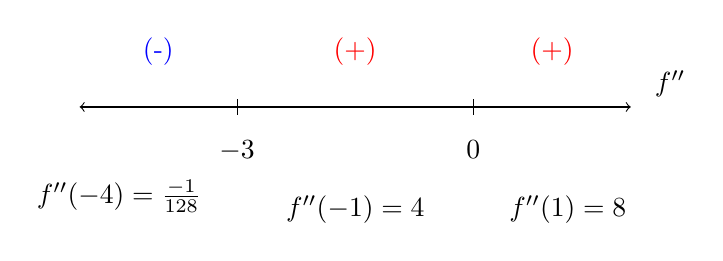
\begin{tikzpicture}
             \draw [<->] (-5,0) -- (2,0);
             \draw (0,0.1) -- (0,-0.1);
             \draw (-3,0.1) -- (-3,-0.1);
             \draw (-3,-0.3)node[below]{$-3$};
             \draw (0,-0.3)node[below]{$0$};
             \draw (-4.5,-0.8)node[below]{$f''(-4) = \frac{-1}{128}$};
             \draw (-1.5,-1)node[below]{$f''(-1) = 4$};
             \draw (1.2,-1)node[below]{$f''(1) = 8$};
             \draw[red] (-1.5,1)node[below]{(+)};
             \draw[red] (1,1)node[below]{(+)};
             \draw[blue] (-4,1)node[below]{(-)};
             \draw (2.5,0)node[above]{$f''$};
           \end{tikzpicture}
         \end{image}
       \end{center}

       So we see that $f$ is concave up on $(-3,0) \cup (0,\infty)$, and $f$ is concave down on $(-\infty, -3)$.
     \item
       \dfn{Inflection Points}  \\
       $f''(x)$ changes sign from negative to positive at $x=-3$, and $f$ is continuous at $x=-3$.
       So $f$ has an inflection point at $\left( -3, \frac{7}{9} \right)$
			
       \newpage

     \item
       \dfn{The graph of $f$}
       \begin{image}
         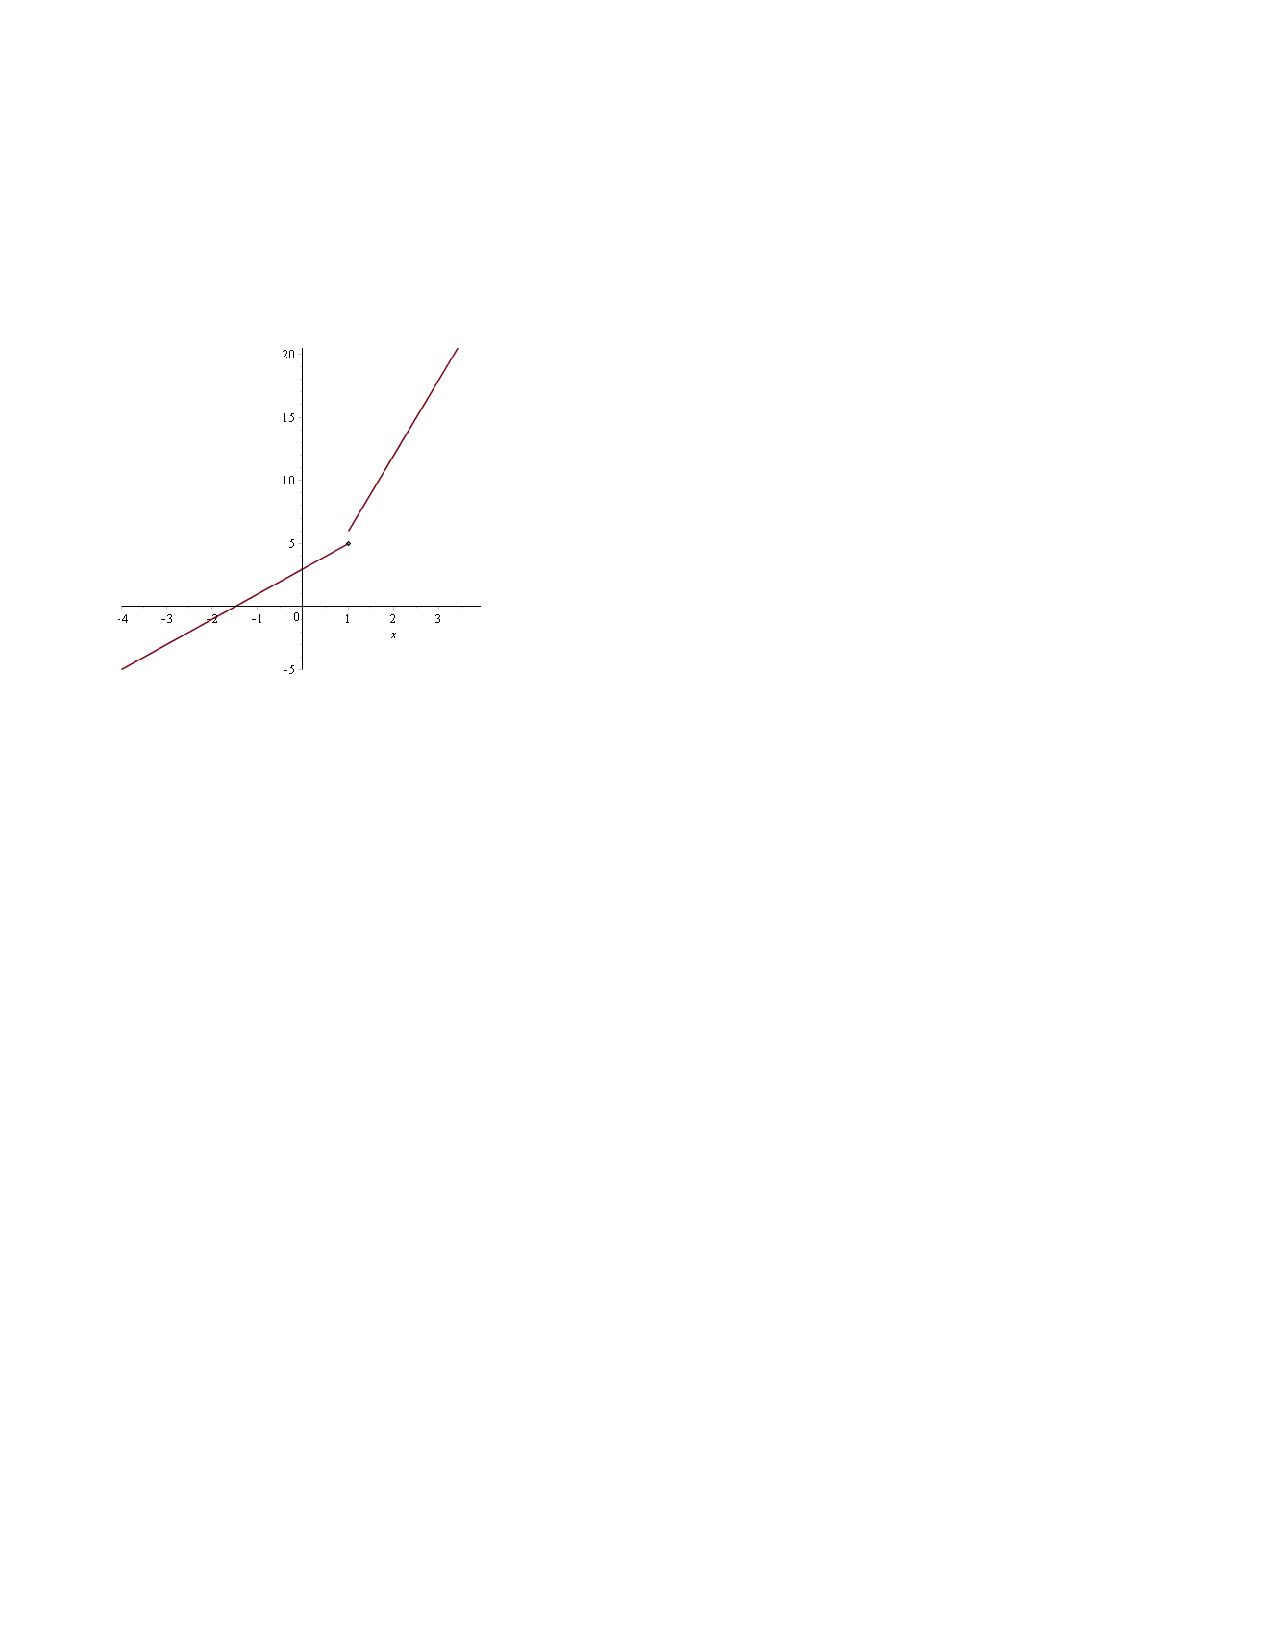
\includegraphics[trim= 220 330 250 180]{Images/Figure6.pdf}
       \end{image}

    \end{itemize}
  \end{freeResponse}
\end{problem}

\section{Extra problem for personal practice}
\begin{problem}
  Given that:
  \[
    \lim_{x \to - \infty} f(x) = 0 \, , \, \lim_{x \to -3^-} f(x) = \infty \, , \, \lim_{x \to -3^+} f(x) = - \infty \, , \, \lim_{x \to 4^-} f(x) = \infty
  \]
  \[ 
  \lim_{x \to 4^+} f(x) = -\infty \, , \, f(1) = 1 \, , \, f(5) = -2 \, , \, f(-3) \text{ is undefined} \, , \, f(4) \text{ is undefined}
  \]
  \[
  f(9) \text{ is undefined} \, , \, f \text{ is continuous except at } x=-3, 4, \text{ and } 9 
  \]
  \[
    f'(1) \ne 0\, ,f'(7) = 0 \, , \, f'(x) = 2 \text{ for } x > 9 \, , \, f''(1) = 0
  \]
  and the following sign chart for the first and second derivatives of $f$:
  \begin{image}
    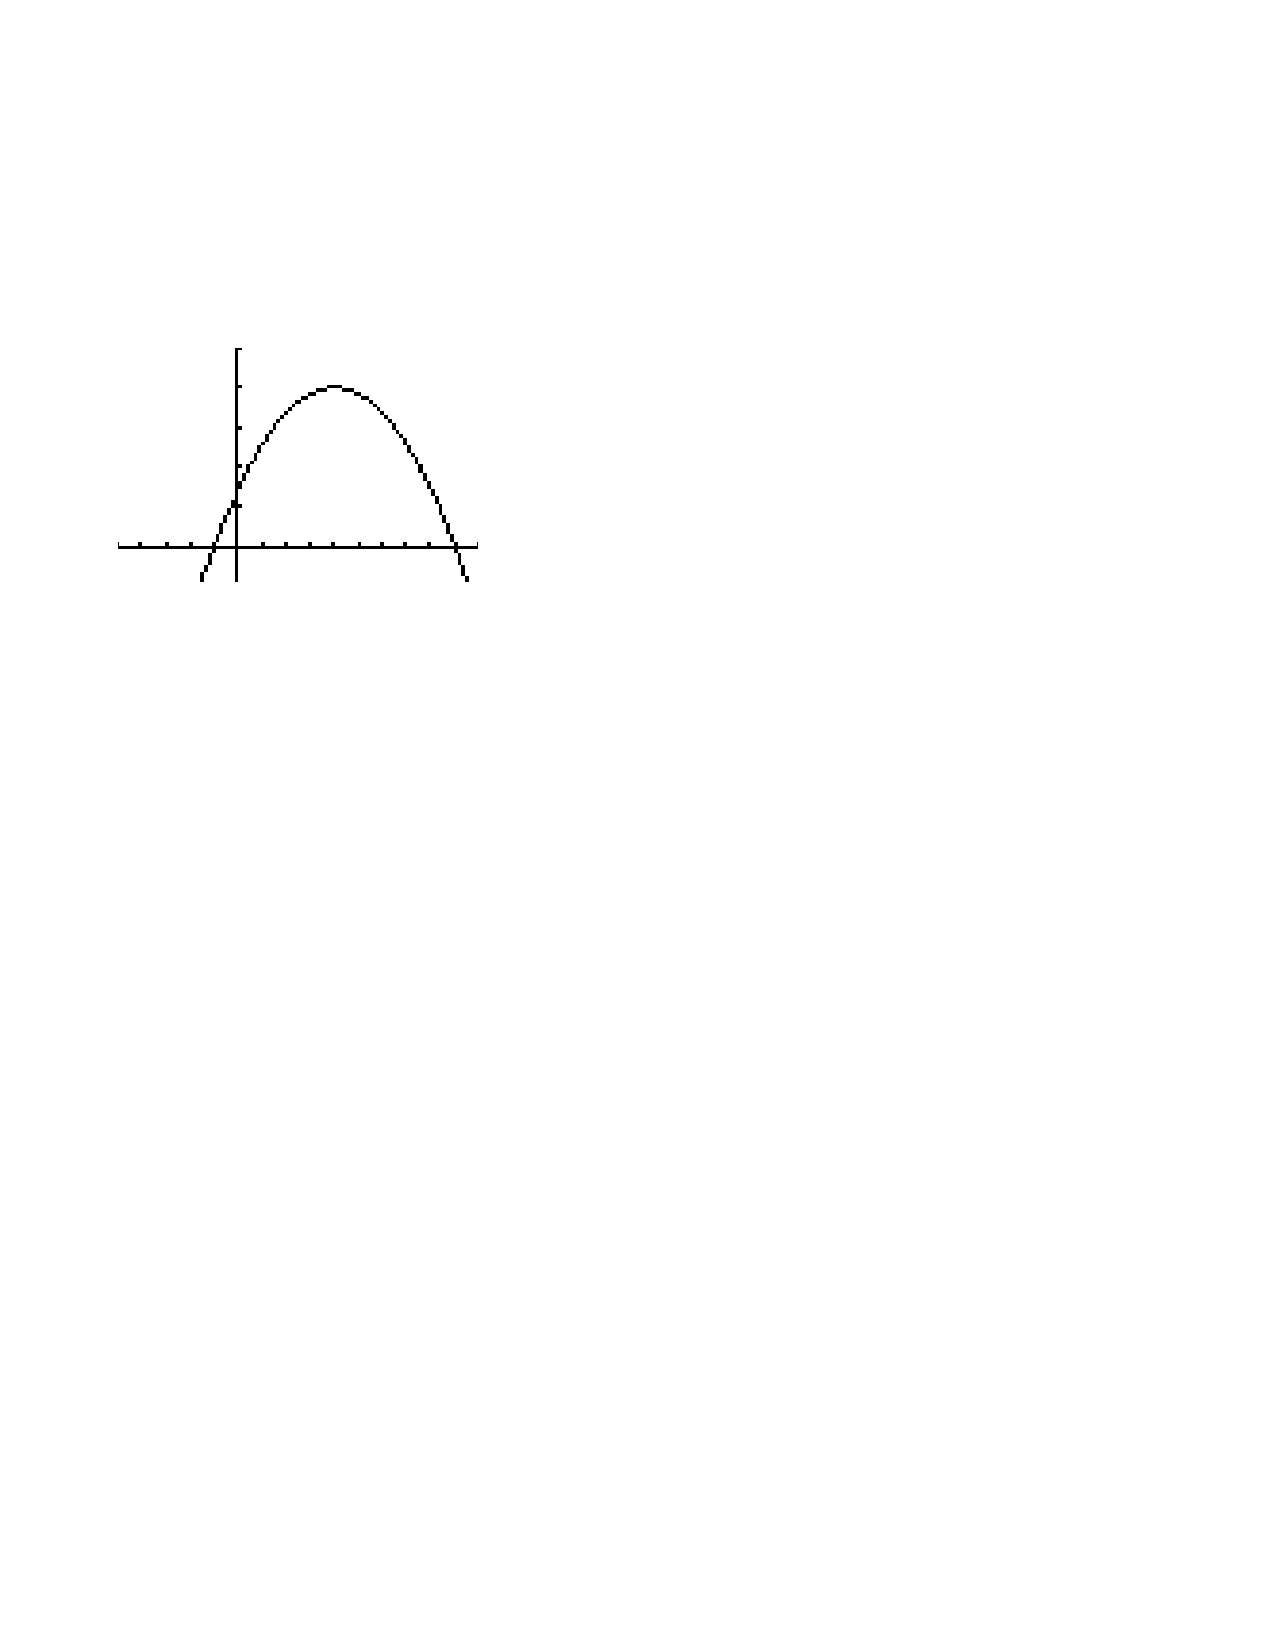
\includegraphics[trim= 70 530 250 190]{Images/Figure4.pdf}
  \end{image}
	
find the following:
  \begin{enumerate}
     \item  Critical points.
     \item  Intervals where $f$ is increasing and decreasing.
     \item  Local extrema.
     \item  Inflection points.
     \item  Intervals of concavity.
     \item  Sketch the graph of $f$.
	
  \end{enumerate}
  \begin{freeResponse}
    \begin{enumerate}
      \item
        Critical points. \\
	The critical points of $f$ occur at points in the domain of $f$ where either $f'(x)=0$ or where $f'(x)$ does not exist.
        We are given that $f'(7)=0$, and so $x=7$ is a critical point of $f$.
        Even though $f'(-3), f'(4),$ and $f'(9)$ do not exist, all three of those points are not in the domain of $f$.
        Therefore, $x=7$ is the only critical point of $f$.  
			
      \item
        Intervals where $f$ is increasing and decreasing.  \\
        $f$ is increasing when $f'(x)>0$.
        From the sign chart and our critical points, these are the intervals $(-\infty ,-3)$, $(-3,4)$, $(4,7]$, and $(9,\infty )$.
        $f(x)$ is decreasing when $f'(x)<0$.
        From the sign chart, this is on the interval $[7,9)$.
			
      \item
        Local extrema.  \\
        Using the first derivative test, $f(7)$ is a local maximum because the derivative changes sign from positive to negative.
        Although the derivative changes sign from negative to positive at $f(9)$, this is not a local minimum because the function is not defined at this point.
        Therefore, $x=7$ is the only local extremum of $f$, and it is a local maximum.
			
      \item
        Inflection points.  \\
        Possible inflection points occur where $f''(x)=0$ or where $f''(x)$ does not exist.
        We are given that $f''(1)=0$.
        In addition, $f''(x)$ does not exist at $x=-3,4,9$.
        However, these are not inflection points because $f$ is not defined at these points.
        Since $f''$ changes sign at $x=1$, this is in fact an inflection point of $f$.
        We are given that $f(1) = 1$, and so the only inflection point of $f$ is the point $(1,1)$.  
			
      \item
        Intervals of concavity.  \\
        $f(x)$ is concave up when $f''(x)>0$.
        From the sign chart, this is on the intervals $(-\infty ,-3)$ and $(1,4)$.
        $f(x)$ is concave down when $f''(x)<0$.
        From the sign chart, this is on the interval $(-3,1)$ and $(4,9)$.
        
			
      \item
        Sketch the graph of $f$.
        \begin{image}
          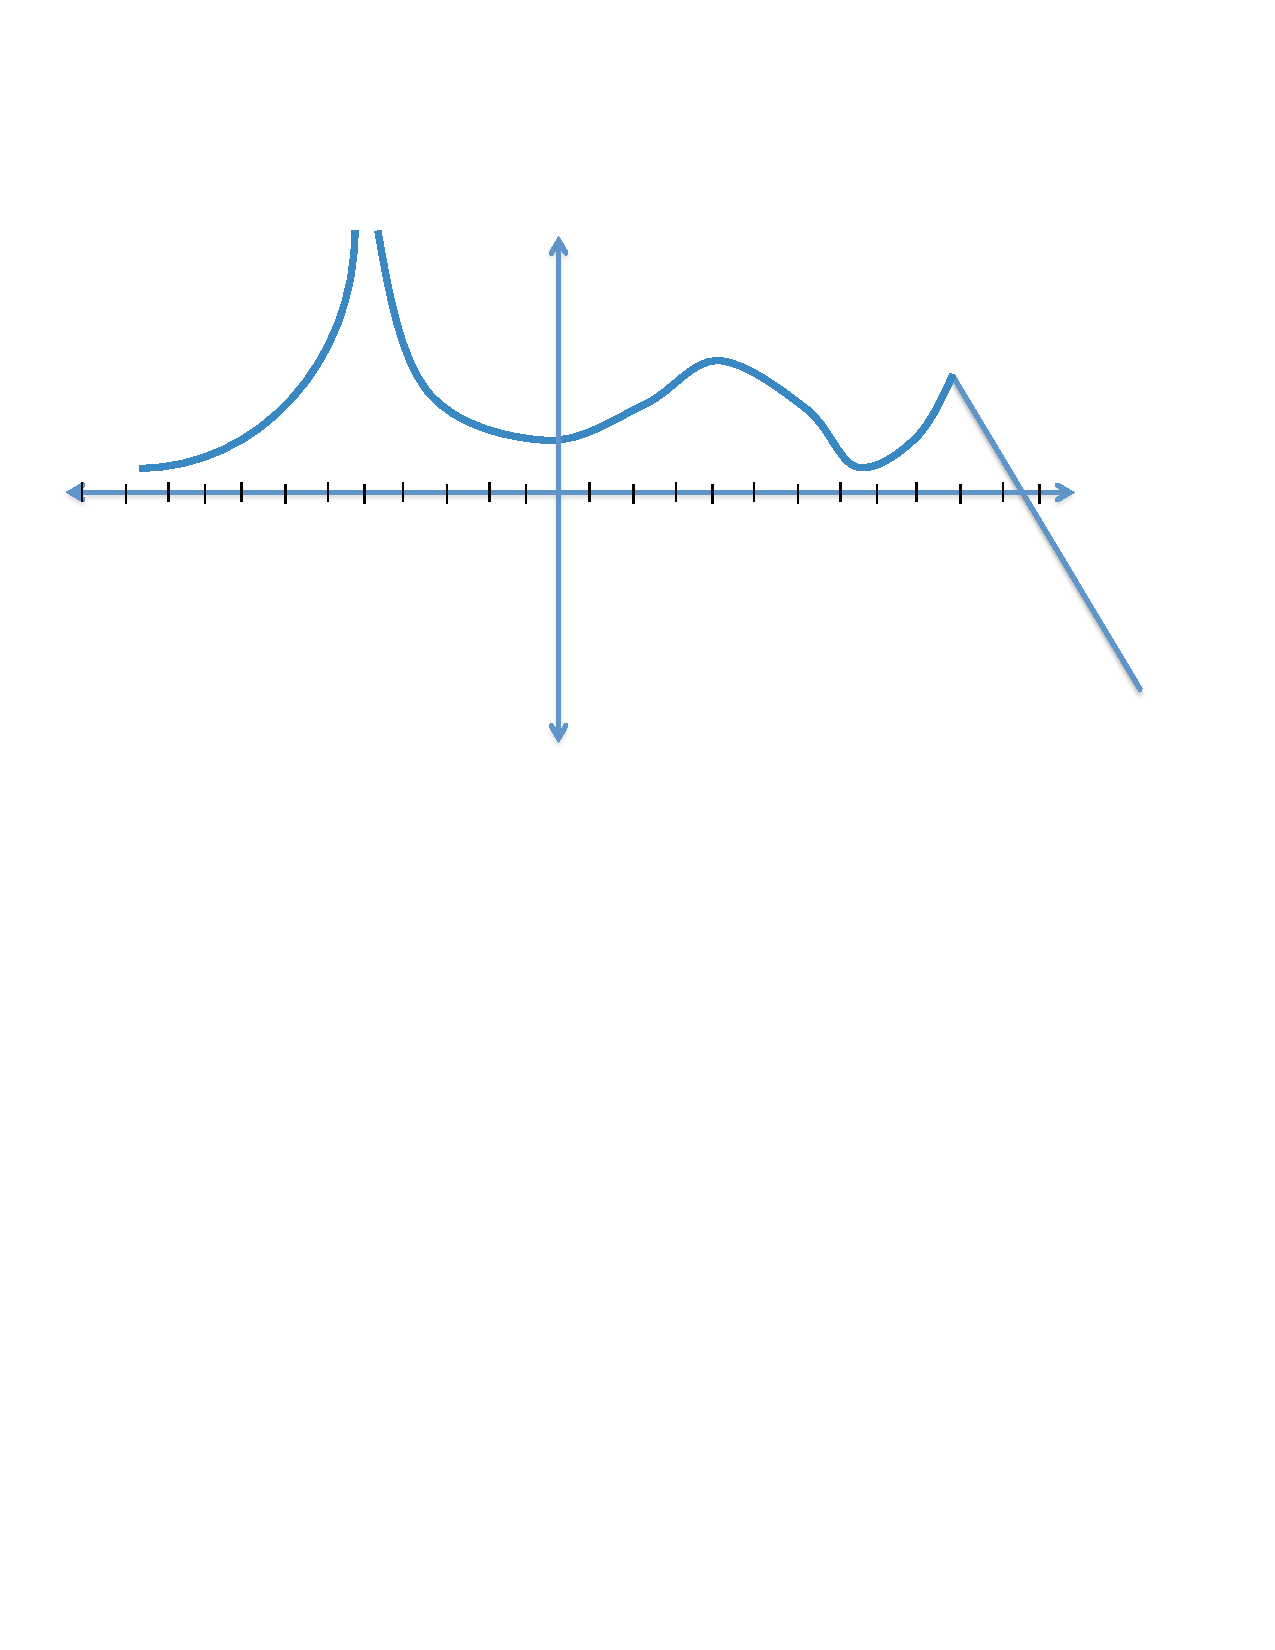
\includegraphics[trim= 220 530 250 120]{Images/Figure5.pdf}
	\end{image}
    \end{enumerate}
  \end{freeResponse}
\end{problem}
\newpage
\begin{center}  \dfn{Graph Sketching Summary Sheet}  \end{center}

\begin{enumerate}

\item[1.]  \dfn{Domain}  \\
	Find the domain of the function $f$.

\item[2.]  \dfn{$x, \, y$ - intercepts}
	\begin{itemize}
		\item $x$-int: set $f(x)=0$ and solve for $x$.
		\item $y$-int: plug in 0 for $x$ and solve for $y$.
	\end{itemize}

\item[3.]  \dfn{Symmetry} 
	\begin{itemize}
		\item  Odd:  $f(-x)=-f(x)$, symmetric about the origin.
		\item  Even:  $f(-x)=f(x)$, symmetric about the y-axis.
		\item  Periodic:  $f(x+k)=f(x)$ for all x, period is k.
	\end{itemize}

\item[4.]  \dfn{Asymptotes} 
	\begin{itemize}
		\item  Vertical Asymptotes:  lines $x=a$ where either $\lim_{x \to a^-} f(x) = \pm \infty$ or $\lim_{x \to a^+} f(x) = \pm \infty$.
		\item  Horizontal Asymptotes:  lines $y=b$ where either $\lim_{x \to \infty} f(x) = b $ or $\lim_{x \to -\infty} f(x) = b $.
	\end{itemize}
	
\item[5.]  \dfn{Increasing/decreasing}
	\begin{itemize}
		\item  $f'(x) > 0 \quad \Longrightarrow \quad f$ is increasing.
		\item  $f'(x) < 0 \quad \Longrightarrow \quad f$ is decreasing.
	\end{itemize}
\item[6.]  \dfn{Maxima/Minima}  \\
	Use the First and/or Second Derivative Test(s) to determine whether a critical point of $f$ is a local maximum, minimum, or neither.
	
\item[7.]  \dfn{Concavity}
	\begin{itemize}
		\item  $f''(x) > 0 \quad \Longrightarrow \quad f$ is concave up.
		\item  $f''(x) < 0 \quad \Longrightarrow \quad f$ is concave down.
	\end{itemize}

\item[8.]  \dfn{Inflection Points}  \\
	$x=a$ is an inflection point of $f$ if BOTH $f''(x)$ changes sign at $x=a$ AND $f$ is continuous at $x=a$.
\end{enumerate}




\end{document} 
